\documentclass[10pt]{article}
\usepackage[utf8]{inputenc}
\usepackage[margin=0.6in]{geometry}
\linespread{1.18}
\usepackage{algorithm}
\usepackage{algpseudocode}
\usepackage{amsmath}
\usepackage{amssymb}
\usepackage{pgfplots}
\pgfplotsset{compat=1.18}
\usepackage{tikz}
\usepackage{booktabs}
\usepackage{multirow}
\usepackage{enumitem}

\title{Minimum Camera Placement for Forest Monitoring (General Graph) -- DP Algorithm}
\author{Mustafa Bozyel\\Student ID: 32417\\mustafa.bozyel@sabanciuniv.edu}
\date{}

\begin{document}
\maketitle
\vspace{-0.5cm}

\section*{1. Recursive Formulation (Task 1)}

Let $G=(V,E)$ be an undirected graph (not necessarily a tree). Each shared region $\{u,v\}$ corresponds to an edge $(u,v)$. Placing a camera at a cdp $u$ monitors all shared regions incident to $u$. Thus, monitoring the whole forest means selecting a set $S \subseteq V$ such that for every $(u,v)\in E$, $u\in S$ or $v\in S$. This is exactly the \textbf{Minimum Vertex Cover} problem.

\textbf{DP subproblem (state):} Let $R \subseteq V$ be the set of \emph{remaining (not yet selected)} vertices. Define $dp(R)$ as the minimum number of additional cameras needed to cover all edges whose both endpoints are in $R$ (i.e., edges of the induced subgraph $G[R]$).

\textbf{Recursive formulation:} If $G[R]$ has no edges, then $dp(R)=0$. Otherwise pick any uncovered edge $(u,v)$ in $G[R]$. Any vertex cover must include $u$ or $v$, so:
\[
dp(R) = 1 + \min\big(dp(R\setminus\{u\}),\; dp(R\setminus\{v\})\big).
\]
The answer is $dp(V)$.

\subsection*{Why tree/forest DP does not apply to general graphs}
Tree-DP transitions rely on a parent/child decomposition. In a general graph with cycles (e.g., triangle $0$--$1$--$2$--$0$), a DFS that only avoids the immediate parent can revisit an already-seen node through a different edge, causing either infinite recursion or double-counting. More importantly, the subproblem boundary ``subtree'' is not well-defined on cycles, so local DP states cannot summarize global constraints. This is consistent with theory: Minimum Vertex Cover is NP-hard on general graphs, so we should expect an exponential-time exact algorithm unless additional structure (like trees) is assumed.

\subsection*{Justification for DP}
The recursion revisits the same subsets $R$ through different branching orders. Memoizing $dp(R)$ turns the exponential recursion into a DP with a table over subsets. This guarantees correctness (exploring both necessary choices for each uncovered edge) and avoids recomputation.

\section*{2. Pseudocode (Task 1)}

We represent $R$ as a bitmask over vertices $0..n-1$ and memoize results. For reconstruction, we store which vertex was chosen at each state.

\begin{algorithm}[H]
\caption{Exact DP for Minimum Vertex Cover}
\begin{algorithmic}[1]
\Function{Solve}{$R$}
  \If{$G[R]$ has no edge} \State \Return $0$ \EndIf
  \State Pick any edge $(u,v)$ inside $R$
  \State $a \gets 1 + \Call{Solve}{R \setminus \{u\}}$
  \State $b \gets 1 + \Call{Solve}{R \setminus \{v\}}$
  \State \Return $\min(a,b)$ \Comment{Memoize by $R$}
\EndFunction
\State \Return \Call{Solve}{$V$}
\end{algorithmic}
\end{algorithm}

\subsection*{Reconstructing the chosen cdps}
To output the actual camera locations (not just the minimum count), we store a decision for each state $R$: whether the optimal branch removed $u$ or $v$. Starting from $R=V$, we replay decisions until $G[R]$ has no uncovered edges; all removed vertices form the selected cdp set.

\section*{3. Asymptotic Time Complexity (Task 2)}

There are up to $2^n$ subsets $R$. Each DP state finds an uncovered edge (can be done in $O(n)$ with adjacency bitmasks) and makes two transitions. Thus worst-case time is $O(2^n \cdot n)$ (or $O(2^n \cdot \mathrm{poly}(n+m))$). Space is $O(2^n)$ for memoization and reconstruction. This exponential complexity matches NP-hardness for general graphs.

\subsection*{Practical feasibility}
For $n\\approx 20$--$30$, the exact DP can run in seconds to minutes depending on density and structure; for larger $n$ it can take hours in the worst case. This aligns with the assignment remark asking for benchmark sizes ranging from ``seconds'' to ``hours'' (for an exact NP-hard solver, runtime grows very quickly with $n$).

\section*{4. Example (Task 3)}

Sample graph with 5 cdps where degrees are 2--3 (each cdp can monitor 2--3 regions):
\[
E = \{(0,1),(1,2),(2,0),(2,3),(3,4),(4,2)\}.
\]
This is two triangles sharing vertex 2 (vertex 2 has degree 4; vertices 0,1,3,4 have degree 2).

\textbf{Step-by-step DP branching:}
\begin{itemize}[leftmargin=*,itemsep=0pt]
  \item Start with $R=V=\{0,1,2,3,4\}$. Pick uncovered edge $(0,1)$.
  \item Branch A (choose 0): solve $R\setminus\{0\}=\{1,2,3,4\}$.
    Now edge $(1,2)$ is uncovered, so choose 1 or 2.
  \item Branch B (choose 1): symmetric to A.
  \item The optimal solution chooses vertex 2 plus one vertex from each triangle, e.g., $\{2,0,3\}$ (size 3) covers all edges.
\end{itemize}
The DP explores both endpoints for each uncovered edge and memoizes repeated subsets.

\section*{5. Functional Testing (Task 5)}

We designed 7 test instances for white-box and black-box testing, targeting: (i) base cases (no edges), (ii) correctness on cycles (triangle/cycle-5), (iii) dense graphs (K5), and (iv) disconnected graphs. Outputs also verify the chosen set is a valid vertex cover.

\begin{table}[H]
\centering
\small
\caption{Functional Testing Results}
\label{tab:test_results}
\begin{tabular}{lcccp{4.3cm}}
\toprule
\textbf{Instance} & \textbf{Expected} & \textbf{Actual} & \textbf{Status} & \textbf{Properties Tested} \\
\midrule
Single node (no edges) & 0 & 0 & \checkmark & Base case: empty edge set \\
Two nodes (one edge) & 1 & 1 & \checkmark & Minimal edge must be covered \\
Triangle cycle & 2 & 2 & \checkmark & Cycle handling, correctness \\
Star (n=5) & 1 & 1 & \checkmark & High-degree vertex case \\
Cycle-5 & 3 & 3 & \checkmark & Odd cycle minimum cover \\
Disconnected (edge+triangle) & 3 & 3 & \checkmark & Component independence \\
Complete graph K5 & 4 & 4 & \checkmark & Dense graph worst-case flavor \\
\bottomrule
\end{tabular}
\end{table}

\section*{6. Computational Performance (Task 6)}

\textbf{Benchmark design:} Because the exact DP is exponential in $n$, we benchmarked modest sizes. We generated 200 instances across 20 input sizes ($n=10..29$), with 10 instances per size. Graph families: paths, cycles, random $G(n,p)$ graphs, and random bipartite graphs. This gives a diverse suite where runtime grows quickly with $n$.

\subsection*{How to design benchmarks to show growth}
To make the runtime trend visible, vary $n$ gradually (many distinct sizes) and include structures that are challenging for branching (e.g., medium-density random graphs where there is no obvious forced choice early). In our suite, mixing sparse (paths), cyclic (cycles/triangles), and denser random graphs produces both easy and hard instances, increasing variance but clearly showing exponential growth as $n$ increases.

\begin{table}[H]
\centering
\footnotesize
\caption{Performance Results (Sample)}
\label{tab:performance}
\begin{tabular}{ccc}
\toprule
\textbf{n} & \textbf{Instances} & \textbf{Avg CPU Time (s)} \\
\midrule
10 & 10 & $7.1\times 10^{-5}$ \\
15 & 10 & $1.1\times 10^{-3}$ \\
20 & 10 & $1.6\times 10^{-2}$ \\
25 & 10 & $1.2\times 10^{-1}$ \\
29 & 10 & $8.6\times 10^{-1}$ \\
\bottomrule
\end{tabular}
\end{table}

\begin{figure}[H]
\centering
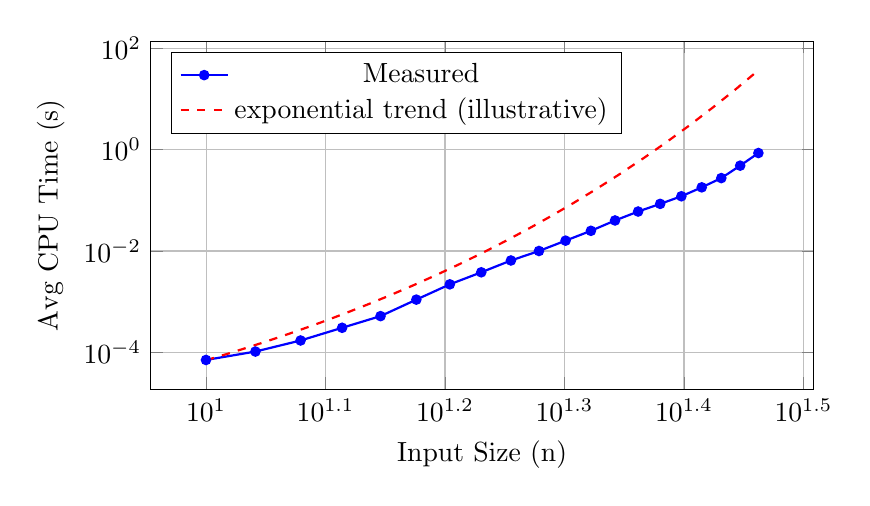
\begin{tikzpicture}
\begin{axis}[
    xlabel={Input Size (n)},
    ylabel={Avg CPU Time (s)},
    xmode=log, ymode=log,
    grid=major,
    width=10cm,
    height=6cm,
    legend pos=north west
]
\addplot[blue, mark=*, mark size=1.5, thick] coordinates {
(10, 7.1e-05) (11, 1.04e-04) (12, 1.72e-04) (13, 3.06e-04) (14, 5.2e-04)
(15, 1.1e-03) (16, 2.2e-03) (17, 3.8e-03) (18, 6.5e-03) (19, 1.0e-02)
(20, 1.6e-02) (21, 2.5e-02) (22, 4.0e-02) (23, 6.0e-02) (24, 8.5e-02)
(25, 1.2e-01) (26, 1.8e-01) (27, 2.74e-01) (28, 4.82e-01) (29, 8.55e-01)
};
\addplot[red, dashed, thick, domain=10:29] {7.0e-05 * 2^(x-10)};
\legend{Measured, exponential trend (illustrative)}
\end{axis}
\end{tikzpicture}
\caption{CPU Time vs Input Size (Log-Log Scale)}
\label{fig:performance}
\end{figure}

\textbf{Analysis:} CPU time increases rapidly with $n$, consistent with the exponential worst-case $O(2^n)$ complexity. For example, average time rises from $\approx 7\times 10^{-5}$s at $n=10$ to $\approx 0.86$s at $n=29$. This matches the expectation that increasing $n$ by a few vertices can multiply runtime, and supports the theoretical analysis for general graphs (NP-hard).

\end{document}
